\section{The Main Idea}

\begin{figure}[t]
\begin{center}
\epsfig{file=arch.eps, width=0.7\columnwidth}
\caption{The architecture}\label{fig-idea}
\end{center}
\end{figure}

%\begin{figure}[t]
%\begin{center}
%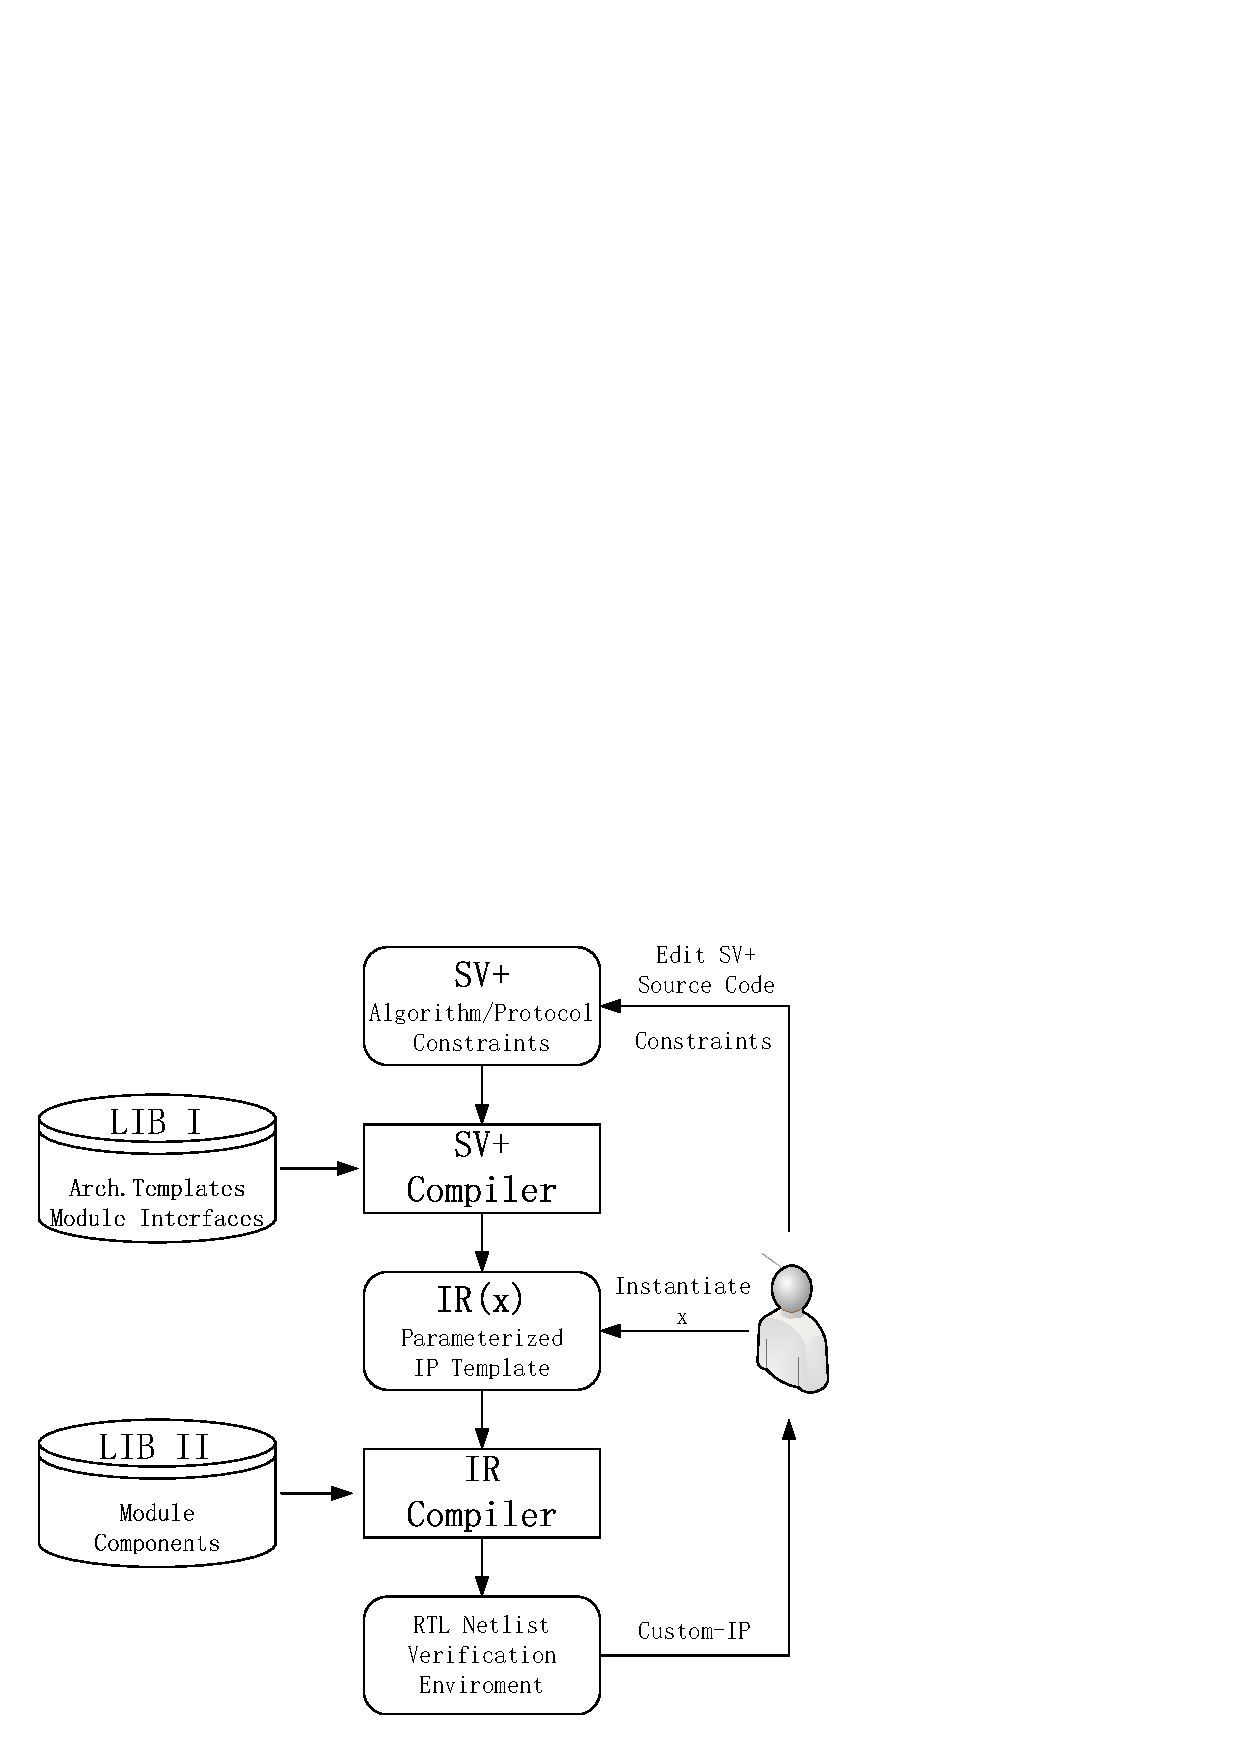
\includegraphics{arch.gif}
%\caption{The architecture}\label{fig-idea}
%\end{figure}


Figure \ref{fig-idea} depicts the architecture of the proposed the RICH system. 
The IP designer describes the algorithm, IP interfaces as well as constraints in SV+, 
a language extension to SystemVerilog. 
The constrains define the physical properties of IP, such as maximum frequency, area cost, or minimum throughput.
The SV+ code then gets preprocessed by an SV+ preprocessor.
This is a coarse-grained IP generation step in which the preprocessor searches
through the {\em template library} to locate most suitable hardware templates that satisfies the
IP constraints and module interfaces. The result of the preprocessing is a parameterized 
intermediate representation of the algorithm, IR($x$),  where $x$ is a set of variable parameters. 
At this point, the designer instantiate these variables using a configuration file. 
Finally, in a fine-grained IP generation step, the fully
instantiated IR is compiled into the RTL and verification environment with
the help of the module library. The end result of the entire flow is a custom IP core, 
and it is passed to the designer for verification.
In case the generated custom IP core does not match the specification, 
the designer can modify his or her design by either fine tuning the IR with a different set of variable
instantiations, or by coarse adjustment in the SV+ code.
The template library is designed for mapping algorithms to specific hardware architectures. 
It is co-designed by hardware engineers and algorithm designers, and it is highly optimized for 
hardware implementation. 
The module library contains many frequently used module components. 
The circuit-level optimizations are accomplished both in this library and during RTL code generation. 
Both libraries are open and extendable, which makes the system highly flexible. 


%
%\begin{enumerate}
%\item Algorithm or protocol description and constrains definition. 
%      User describes the algorithm and IP interface by a high-level language, such as SystemVerilog with extension (SV+). 
%      The constrains define the physical properties of IP, such as maximum frequency, area cost, or minimum throughput.  
%\item SV+ preprocessor. 
%      It can be considered as a coarse IP generation step. 
%      In this step, the preprocessor searches and optimizes the existing hardware architecture template and 
%      the module interfaces in the library to find a proper hardware template to satisfy the IP constraints.  
%\item Intermediate Representation (IR) of an IP core. 
%      IR(x) is a parameterized representation of an IP core. 
%      x represents some configurable variables in IP core. 
%      In order to generate different IP cores, user should instantiate these variables. 
%\item IR compiler. 
%      It can be considered as a fine IP generation step. 
%      Based on the specific hardware template, user-input configurations, 
%      and the detailed hardware implementations of each module components in library, 
%      R compiler will generate the final rtl codes for IP cores.  
%\item Output. 
%      The final output includes RTL netlist and the corresponding verification environment, which also can be called as custom-IP core.
%\end{enumerate}

